% \begin{example}
%   \label{antipattern:example:contrib_variant}
%   The following rewriting rule is obtained from a rewriting rule in~\cite[Example 6]{plump2018modular} by removing all edges of the interface graph and adding a node with the identifier $5$ and three self-loops labeled $0$ to the right-hand-side graph.
%   \begin{center}
%       \resizebox{0.8\textwidth}{!}{
%           \begin{tikzpicture}
%               \graphbox{$L$}{0mm}{0mm}{35mm}{35mm}{2mm}{-5mm}{
%                   \coordinate (delta) at (0,-18mm);
%                   \node[draw,circle] (l1) at ($(delta)+(-1,1.5)$) {1};
%                   \node[draw,circle] (l2) at ($(delta)+(1,1.5)$) {2};
%                   \node[draw,circle] (l3) at ($(delta)+(0,0)$) {3};
%                   \draw[->] (l1) -- (l3) node[midway,left] {$s$};
%                   \draw[->] (l2) -- (l3) node[midway,right] {$s$};
%                   \draw[->] (l3) edge [loop below] node {0} (l3);
%               }
%               \graphbox{$K$}{40mm}{0mm}{35mm}{35mm}{2mm}{-5mm}{
%                   \coordinate (delta) at (0,-18mm);
%                   \coordinate (interfaceorigin) at ($(delta) +(5,0)$);
%                   \node[draw,circle] (r1) at ($(delta) +(-1,1.5)$) {1};
%                   \node[draw,circle] (r2) at ($(delta) +(0.5,1.5)$) {2};
%                   \node[draw,circle] (r3) at ($(delta)+(0,0)$) {3};
%               }
%               \graphbox{$R$}{80mm}{0mm}{50mm}{35mm}{2mm}{-5mm}{
%                   \coordinate (delta) at (-10mm,-18mm);
%                   \node[draw,circle] (r1) at ($(delta)+(-1,1.5)$) {1};
%                   \node[draw,circle] (r2) at ($(delta)+(0.5,1.5)$) {2};
%                   \node[draw,circle] (r3) at ($(delta)+(0,0)$) {3};
%                   \node[draw,circle] (r4) at ($(delta)+(1,0)$) {4};
%                   \draw[->] (r1) -- (r3) node[midway,left] {$s$};
%                   \draw[->] (r2) -- (r4) node[midway,right] {$s$};
%                   \draw[->] (r4) edge [loop below] node {0} (r4);
%                   \draw[->] (r3) edge [loop below] node {0} (r3);
%                   \node[draw,circle] (r5) at ($(r2)+(1.5,0)$) {5};
%                   \draw[->] (r5) edge [loop below] node {0} (r5);
%                   \draw[->] (r5) edge [loop right] node {0} (r5);
%                   \draw[->] (r5) edge [loop left] node {0} (r5);
%               }
%               \node () at (38mm,-18mm) {$\leftarrowtail$};
%               \node () at (77mm,-18mm) {$\rightarrowtail$};
%           \end{tikzpicture}
%           }
%         \end{center}
  
%       Consider the ruler-graph $\mathcal{X} \mathop{=} (X)$, where $X$ is the graph
%       \tikz[baseline=-0.5ex]{ 
%               \node[draw,circle] (x) at (0,0) { }; 
%               \node[draw,circle] (y) at (1,0) { };
%               \node[draw,circle] (z) at (2,0) { };
%               \draw[->] (x) -- (y) node[midway, above] {$s$};
%               \draw[->] (z) -- (y) node[midway, above] {$s$};
%       } and there is no forbidden context. $\mathcal{X}$ has weight $1$ and $\mathbb{X} \mathop{=} \{X\}$.
%       The set \( D(R,X) \) contains a unique element $R'$:
%       \raisebox{2pt}{
%           \scalebox{0.7}{\tikz[baseline=-0.5ex]{
%           \node [draw,circle] (x) at (0,0) {1};
%           \node[draw,circle] (y) at (1,0) {3};
%           \draw[->] (x) -- (y) node[midway, above] {$s$};
%       }}}.
%       \textcolor{red}{The rule is $X$-non-increasing under the function that maps the subgraph $R'$ of $R$ in $R$ to the same subgraph in $L$. }\todo{to do todo:n'importe quoi}
%     %   Since $F_X \mathop{=} \emptyset$, the number of $X$-occurrences not included in any occurrences of forbidden context in any rewriting step is predictable.
%       By Theorem~\ref{antipattern:thm:termination_grs}, the rule terminates because \(|Mono(X,L)| - |Mono(X,R)| \mathop{=} 1 - 0 \mathop{=} 1 \mathop{>} 0 \). 
% \end{example}
\begin{example}
  \label{antipattern:ex:grs_aca}
  Consider the rule $\rho$ shown below.
  \begin{center}
  % \resizebox{0.8\textwidth}{!}{ 
    \begin{tikzpicture}   
        \graphbox{$L$}{0mm}{0mm}{34mm}{20mm}{2mm}{-5mm}{
            \coordinate (o) at (0mm,-3mm); 
            \node[draw,circle] (l1) at ($(o)+(-10mm,0mm)$) {1};
            \node[draw,circle] (l2) at ($(l1)+(2,0)$) {2};
            \node[draw,circle] (l3) at ($(l1)+(1,0)$) {3};
            \draw[->] (l1) -- (l3) node[midway,above] {$a$};
            \draw[->] (l3) -- (l2) node[midway,above] {$a$};
        }     
        \graphbox{$K$}{40mm}{0mm}{24mm}{20mm}{2mm}{-5mm}{
            \coordinate (o) at (5mm,-3mm); 
            \node[draw,circle] (l1) at ($(o)+(-10mm,0mm)$) {1};
            \node[draw,circle] (l2) at ($(l1)+(1,0)$) {2};
            % \node[draw,circle] (l3) at ($(l1)+(1,0)$) {$\ $};
            % \draw[->] (l1) -- (l3) node[midway,above] {$a$};
            % \draw[->] (l3) -- (l2) node[midway,above] {$a$};
        }    
        \graphbox{$R$}{70mm}{0mm}{45mm}{20mm}{2mm}{-5mm}{
          \coordinate (o) at (0mm,-3mm); 
          \node[draw,circle] (l1) at ($(o)+(-10mm,0mm)$) {1};
          \node[draw,circle] (l2) at ($(l1)+(2,0)$) {2};
          \node[draw,circle] (l3) at ($(l1)+(1,0)$) {3};
          \draw[->] (l1) -- (l3) node[midway,above] {$a$};
          \draw[->] (l3) -- (l2) node[midway,above] {$a$};
          \draw[->] (l3) edge [loop below] node {$c$} (l3);
        }    

        \node () at (37mm,-10mm) {$\leftarrowtail$};
        \node () at (67mm,-10mm) {$\rightarrowtail$};

        % \draw[>->] (51mm,2mm) -- (52mm,3mm);
    \end{tikzpicture}
  % }
\end{center}
Consider the ruler-graph $\mathcal{X} \mathop{=} (L, \set{f})$ where the underlying graph is $L$ and $f:L \rightarrowtail R$ is the inclusion function. Let $s_\mathbb{X}$ be the weight function with $s_\mathbb{X}(\mathcal{X})=1$.
% The number of $L$-occurrences not included in any occurrences of the forbidden context $R$ in any rewriting step using this rule is predictable:
% the condition~\ref{hyp:inj_mono_x_l_to_r} is satisfied because $Mono(L,L)_F \mathop{=} \emptyset$; the condition~\ref{hyp:inj_mono_f_l_to_r} is satisfied because $Mono(R,L) \mathop{=} \emptyset$; the conditions~\ref{hyp:x_non_increasing} and~\ref{hyp:f_non_increasing} are satisfied under identity function; the condition~\ref{hyp:f_non_increasing} is satisfied because for the condition~\ref{hyp:f_non_increasing} we employ identity function. 

Since $D(R,X)$ is the empty set, all conditions in Definition~\ref{subgraph_counting:def:creates_more_x_on_the_left} hold, and rule $\rho$ is $X$-non-increasing. 
Similarly, rule $\rho^{-1}$ is $X$-non-increasing and $F$-non-increasing, because $D(L,X) \mathop{=} \emptyset$ and $D(L,R) \mathop{=} \emptyset$. 

We have 
\begin{flalign*}
\Lambda(\mathcal{X},\rho) \overset{\operatorname{def}}{\mathop{=}}&\card{\operatorname{Mono}(X,L)_{\operatorname{NF}}} - 
\card{
    \Gamma(\operatorname{Mono}(\mathcal{X},L)_{\operatorname{NF}})
    }   -
\card{\operatorname{Mono}(X,R)_{\operatorname{NF}}} \\
\mathop{=}&1 - 0 - 0 \\
\mathop{=}&1.
\end{flalign*}
Therefore, $s_\mathbb{X}(\mathcal{X}) * \Lambda(\mathcal{X},\rho) \mathop{=} 1 \mathop{>} 0$, and the rule terminates by Theorem~\ref{antipattern:thm:termination_grs}.
\end{example} 
% Finally, we present a limitation of our approach.
\begin{example}
    \label{antipattern:ex:endrullis:d3:termination}  
    Our method can prove termination of the rewriting rule $\rho$ shown below.
    %  in Figure~\ref{fig:antipattern:ex_endrullis_d3} from~\cite[Example D.3]{endrullis2024generalized_arxiv_v2}.
    \begin{center}
        % \resizebox{0.8\textwidth}{!}{
    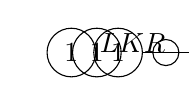
\begin{tikzpicture}  
       \graphbox{$L$}{0mm}{-11mm}{32mm}{15mm}{2mm}{-8mm}{  
           \node[draw,circle]  (x) at (-6mm,0mm) {1};  
           \node[draw,circle]  (y) at (6mm,0mm) {};  
         }  
         \graphbox{$K$}{33mm}{-11mm}{32mm}{15mm}{2mm}{-8mm}{  
           \node[draw,circle]  (x) at (-6mm,0mm) {1};  
         }  
         \graphbox{$R$}{66mm}{-11mm}{32mm}{15mm}{1mm}{-8mm}{  
          \node[draw,circle]  (x) at (-6mm,0mm) {1};  
          \node[draw,circle]  (y) at (6mm,0mm) {};  
          \draw[->]  (x) to (y);  
         }    
   \end{tikzpicture}
    % }
    \end{center}
    Let $\mathcal{X} \mathop{=} (L,\set{f})$ be the ruler-graph where $f:L \rightarrowtail R$ is the unique interface-preserving monomorphism from $L$ to $R$. Let $s_\mathbb{X}$ be the weight function with $s_\mathbb{X}(\mathcal{X})=1$.
    % The number of $X$-occurrences not included in any occurrences of the forbidden context $R$ in any $\rho$-rewriting step is predictable. 
    Since $D(R,X)$ is the empty set, rule $\rho$ is $X$-non-increasing.
    Rule $\rho^{-1}$ is $X$-non-increasing and $R$-non-increasing, because $D(L,X)$ and $D(L,R)$ are empty sets.
    We have 
    \begin{flalign*}
      \Lambda(\mathcal{X},\rho) \overset{\operatorname{def}}{\mathop{=}}&  
      \card{\operatorname{Mono}(X,L)_{\operatorname{NF}}} - 
      \card{ \Gamma(\operatorname{Mono}(\mathcal{X},L)_{\operatorname{NF}})} -
      \card{\operatorname{Mono}(X,R)_{\operatorname{NF}}}
      \\
      \mathop{=}&1 - 0 - 0 
      \\
      \mathop{=}&1.
    \end{flalign*}
    Therefore, $s_\mathbb{X}(\mathcal{X}) * \Lambda(\mathcal{X},\rho) \mathop{=} 1 \mathop{>} 0$, and the rule terminates by Theorem~\ref{antipattern:thm:termination_grs}.
  \end{example} 

% \begin{example}[Limitation]
%   The termination of the rewriting rule presented in~\cite[Ad-hoc routing protocol]{bruggink2014termination} cannot be proven by our method, because the property defined in Definition~\ref{def:predictable} is too restrictive.
% \end{example} 